Linear trap measurements have been taken twice.
The first measurement was with the subcarrier at the same offset frequency from
the carrier for each measurement.
The results generally were in line with the theory, however there were
complications with the layout that we felt should be improved on.

\section{First Experiment}

%\begin{figure}[htbp]
%    \centering
%    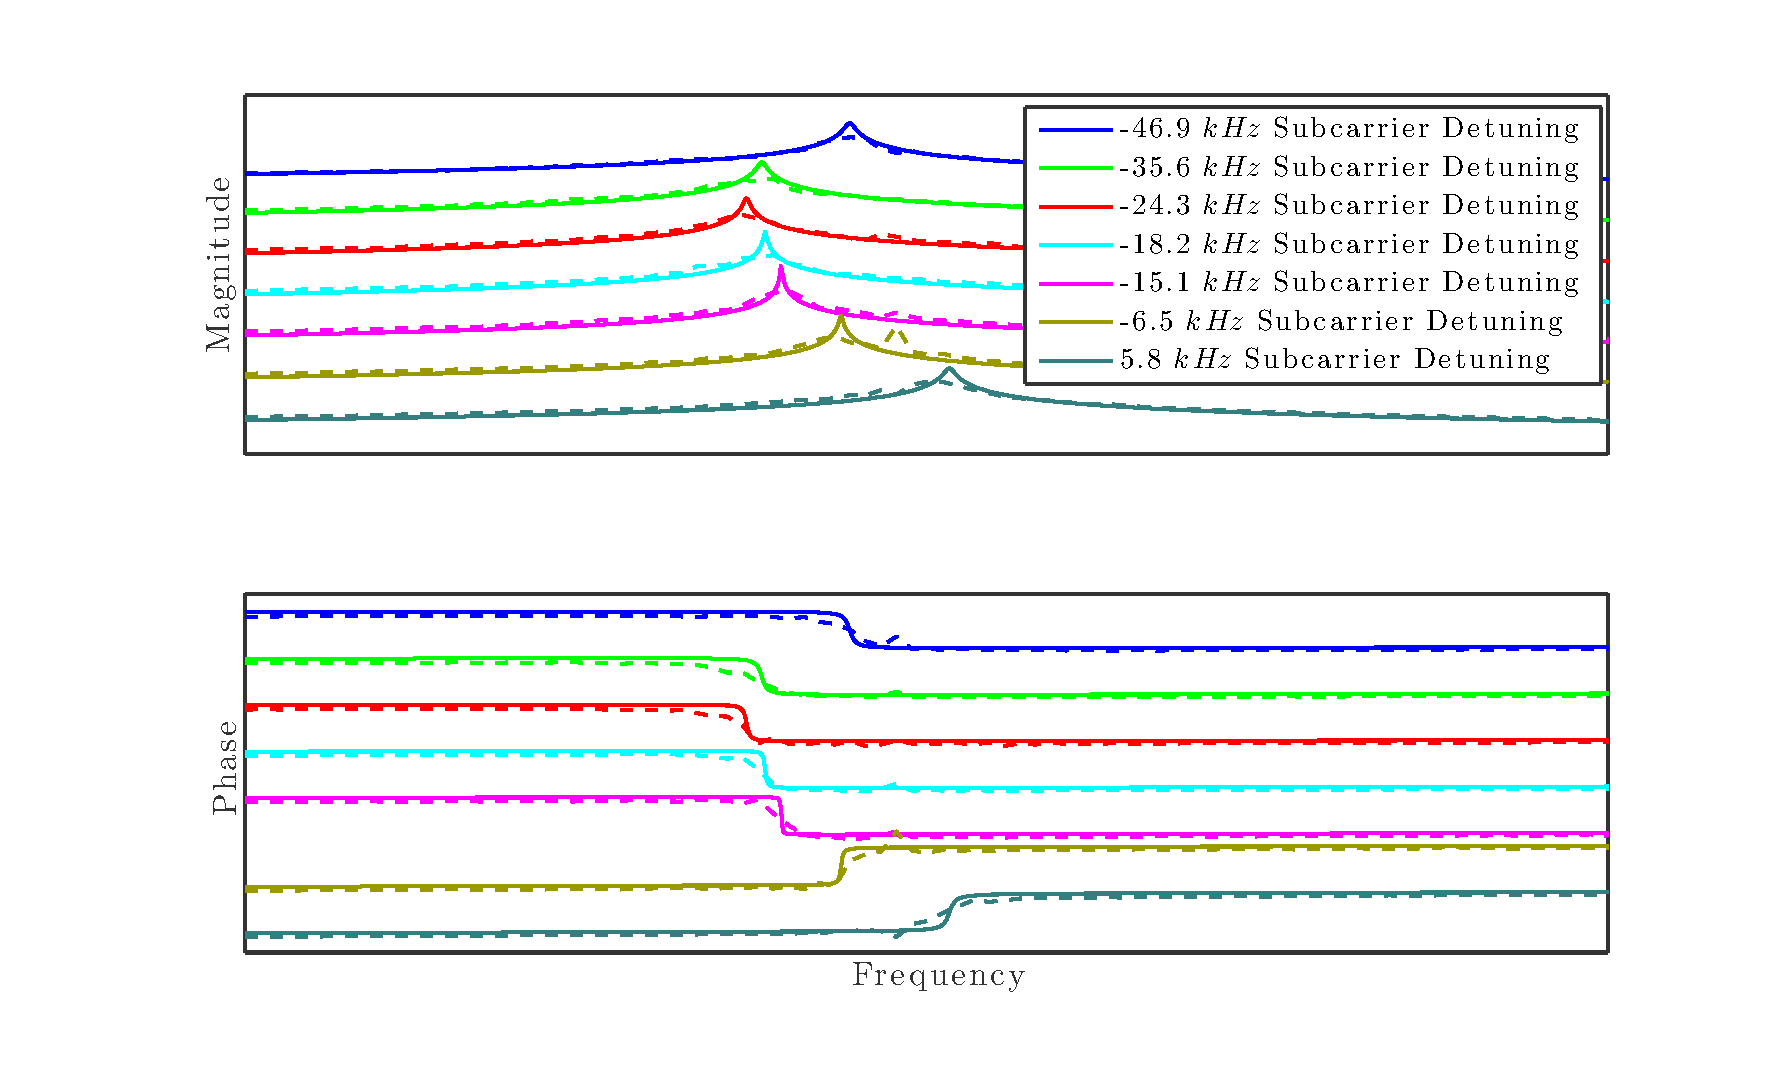
\includegraphics[width=20cm]{./figures/april_results_olgfit.eps}
%    \caption[Data Fitting of Open Loop Gain for 1st Results]{This is the open
%        loop gain fit of the last 7 measurements taken during a segment of
%        time in which the cavity was continuously locked.
%        The trap cavity had been locked for a few hours at this point and
%        seemed to have stabilized compared to earlier in the lock segment.
%        These measurements were taken no more than 5 minutes apart from each
%        other so the effects of any drifted were minimized.}
%    \label{fig:olgapril}
%\end{figure}

\begin{figure}[htbp]
  \tikzsetnextfilename{april_olg1}
  \begin{tikzpicture}
  \begin{semilogyaxis}[
    name=plot1,
    height=6cm,
    xmin=700,
    xmax=900,
    xlabel={Frequency $(kH\!z)$},
    ylabel={Magnitude},
    grid=major,
  ]
  \addplot[blue] table[x index=0,y index=1] {./matlab_traces/april_olg_38.dat};
  \addplot[blue] table[x index=0,y index=1] {./matlab_traces/april_fit.dat};
  \addplot[red] table[x index=0,y index=1] {./matlab_traces/april_olg_39.dat};
  \addplot[red] table[x index=0,y index=3] {./matlab_traces/april_fit.dat};
  \addplot[green] table[x index=0,y index=1] {./matlab_traces/april_olg_40.dat};
  \addplot[green] table[x index=0,y index=5] {./matlab_traces/april_fit.dat};
  \end{semilogyaxis}

  \begin{semilogyaxis}[
    name=plot2,
    at=(plot1.below south), anchor=above north,
    height=6cm,
    xmin=700,
    xmax=900,
    xlabel={Frequency $(kHz)$},
    ylabel={Magnitude},
    grid=major,
  ]
  \addplot[blue] table[x index=0,y index=1] {./matlab_traces/april_olg_41.dat};
  \addplot[blue] table[x index=0,y index=7] {./matlab_traces/april_fit.dat};
  \addplot[red] table[x index=0,y index=1] {./matlab_traces/april_olg_42.dat};
  \addplot[red] table[x index=0,y index=9] {./matlab_traces/april_fit.dat};
  \addplot[green] table[x index=0,y index=1] {./matlab_traces/april_olg_43.dat};
  \addplot[green] table[x index=0,y index=11] {./matlab_traces/april_fit.dat};
  \addplot[black] table[x index=0,y index=1] {./matlab_traces/april_olg_44.dat};
  \addplot[black] table[x index=0,y index=13] {./matlab_traces/april_fit.dat};
  \end{semilogyaxis}
  \end{tikzpicture}
    \caption[Data Fitting of Open Loop Gain for 1st Results]{This is the open
        loop gain fit of the last 7 measurements taken during a segment of
        time in which the cavity was continuously locked.
        The trap cavity had been locked for a few hours at this point and
        seemed to have stabilized compared to earlier in the lock segment.
        These measurements were taken no more than 5 minutes apart from each
        other so the effects of any drifted were minimized.}
  \label{fig:aprilolg1}
\end{figure}
\section{Experimental Layout Revision}
From our first layout design there was a rather
large beat signal on the \ac{rfpd} used for generating the \ac{pdh} signal
for our locking feedback servo.
This beat signal is a result of our initial layout involving the combining of
carrier and subcarrier beams before the \ac{fi} which resulted in the two beams
having the same polarization.
This produces a beat signal of the difference in the two frequencies.
The beat signal shows up in our resonant \ac{rfpd} because we use a small
frequency offset.
We feared there could be saturations in the photodiode electronics that would
cause unpredictable electronic offsets in the trap locking feedback servo
resulting in an error on the subcarrier detuning lock point.



\section{Second Experiment}

